\documentclass{article}
\usepackage{color, colortbl}
\usepackage{amsmath}
\usepackage{graphicx}
\usepackage[a4paper, total={7in, 9in}]{geometry}
\definecolor{LightYellow}{rgb}{255,255,224}
\graphicspath{{images/}}

\title{CCE5225 \dashv{} Assignment 1 \\
\large MiniBooNE particle identification \\ signal/background classification}
\author{Sultan Dayani}
\date{December 2022}
\begin{document}

For all models I used the default parameters except for the ones stated in the text.
\section{Vanilla Neural Network}
\begin{tabular}{|c c c|}
	\hline  
	HL Size & Mean Fit Time & Mean Score \\ [0.5ex] 
	\hline
	(10,) & 99.88s & 0.927113   \\
	\hline
	(20,) & 100.26s & 0.931188   \\
	\hline
	(30,) & 74.61s & 0.933052   \\
	\hline
	(40,) & 376.35s & 0.935090   \\
	\hline
	(50,) & 163.39s & 0.933744   \\ 
  \hline
  (40,) & 75.29s & 0.935311 \\
  \hline
  (40, 40) & 86.75s & 0.936723 \\
  \hline
  (40, 40, 40) & 163.92s & 0.934984 \\
  \hline
  (40, 40, 40, 40) & 249.26s & 0.932158 \\
	\hline
\end{tabular}
% 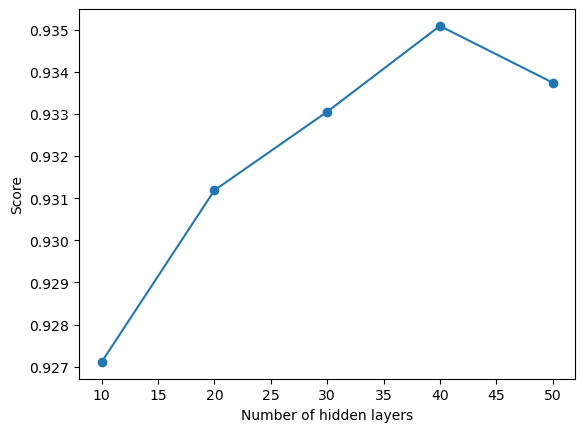
\includegraphics[width=0.6\textwidth]{1hiddenlayer_scores.png}

Using (40,40) and varying the activation function: \\
\begin{tabular}{|c c c|}
	\hline  
	Activation & Mean Fit Time & Mean Score \\ [0.5ex] 
	\hline
  'relu' & 86.75s & test-score: 0.936723 \\ 
	\hline
  'logistic' & 168.04s & test-score: 0.930813 \\ 
	\hline
  'tanh' & 164.20s & test-score: 0.937665 \\ 
	\hline
  'identity' & 41.14s & test-score: 0.893321 \\ 
	\hline
\end{tabular} \\
The activation function 'tanh' gave the best results but took double the time as 'relu'.

Considering the time to train the model,
hidden layer: (30,30), activation: 'relu' results in 101.86s build time and 0.939376 test score, is a good performing one.

\paragraph[Comment]{
The number of hidden layers helps a neural network to learn complex relationships, however too many hidden layers lead to overfitting which reduces performance.
It seems like two hidden layers with 30 neurons lead to a model that understands the relationship of the features well.
The activation functions lie close to each other, I believe the identity functions is the worst performing one as it is a linear function and the data is not linearly separable.
}
\section{SVM}
Except for the stated hyperparameters all others are the default from scikit-learn.
varying C on rbf: \\ 
\begin{tabular}{|c c c|}
C: 0.1 & fit-time: 331.12s & test-score: 0.877185 \\
C: 1 & fit-time: 160.40s & test-score: 0.891601 \\
C: 10 & fit-time: 148.25s & test-score: 0.906661 \\
\end{tabular}
% 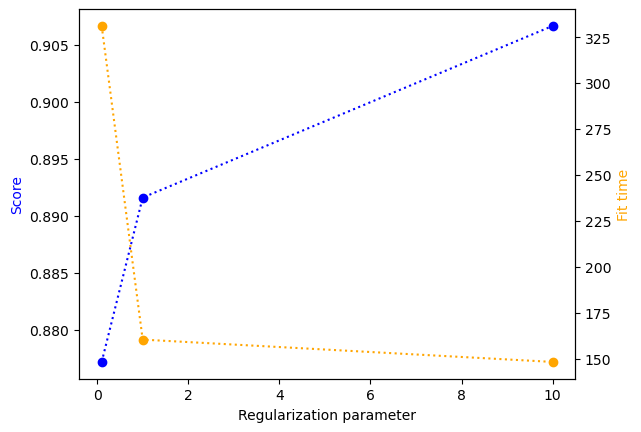
\includegraphics[width=0.6\textwidth]{svm_c_compiled.png}

varying kernel with C=10: \\ 
\begin{tabular}{|c c c|}
% \rowcolor{LightYellow}
kernel: 'rbf' & fit-time: 148.25s & test-score: 0.906661 \\
kernel: 'linear' & fit-time: 463.95s & test-score: 0.904653 \\
kernel: 'poly' & fit-time: 274.41s & test-score: 0.832592 \\
kernel: 'sigmoid' & fit-time: 393.91s & test-score: 0.728335 \\
\end{tabular}
\\ 
The best parameters are: 'C': 10, 'kernel': 'rbf'

\paragraph[Comment]{
Regularization encourages the model to find a balance between complexity and accuracy which lead to a better performing model.
I assume in this example rbf lead to the best results because it does a better job capturing the non-linear relationship between the features and the target.
And also because 'rbf' is tuned by a single hyperparameter and I did not tune the other models hyperparameters.
}

% \pagebreak
\section{Random Forest}
\begin{tabular}{|c c c | c c|}
  \hline  
  Parameters & Fit Time & Test Score \\ [0.5ex] 
  \hline
n-estimators: 50 & min-samples-split: 2 & max-depth: 10 & 22.33s & 0.924643 \\
n-estimators: 50 & min-samples-split: 2 & max-depth: 15 & 30.71s & 0.932408 \\
n-estimators: 50 & min-samples-split: 2 & max-depth: 20 & 36.04s & 0.933984 \\ 
\hline
n-estimators: 50 & min-samples-split: 5 & max-depth: 10 & 22.69s & 0.924575 \\
n-estimators: 50 & min-samples-split: 5 & max-depth: 15 & 30.91s & 0.932860 \\
n-estimators: 50 & min-samples-split: 5 & max-depth: 20 & 35.91s & 0.934388 \\ 
\hline
n-estimators: 50 & min-samples-split: 10 & max-depth: 10 & 22.65s & 0.924864 \\
n-estimators: 50 & min-samples-split: 10 & max-depth: 15 & 31.00s & 0.932552 \\
n-estimators: 50 & min-samples-split: 10 & max-depth: 20 & 35.57s & 0.933110 \\ 
\hline
\hline
n-estimators: 100 & min-samples-split: 2 & max-depth: 10 & 44.06s & 0.924883 \\
n-estimators: 100 & min-samples-split: 2 & max-depth: 15 & 62.45s & 0.933225 \\
n-estimators: 100 & min-samples-split: 2 & max-depth: 20 & 71.87s & 0.934695 \\ 
\hline
n-estimators: 100 & min-samples-split: 5 & max-depth: 10 & 46.42s & 0.925114 \\
n-estimators: 100 & min-samples-split: 5 & max-depth: 15 & 62.23s & 0.933292 \\
n-estimators: 100 & min-samples-split: 5 & max-depth: 20 & 71.88s & 0.935205 \\ 
\hline
n-estimators: 100 & min-samples-split: 10 & max-depth: 10 & 45.57s & 0.925162 \\
n-estimators: 100 & min-samples-split: 10 & max-depth: 15 & 64.83s & 0.933273 \\
n-estimators: 100 & min-samples-split: 10 & max-depth: 20 & 71.10s & 0.934484 \\
\end{tabular}

The best performing model is: 'max-depth': 20, 'min-samples-split': 5, 'n-estimators': 100 with a fit time of 71.88s and a test score of 0.935205.
Considering the time to train the model a random forest with n-estimators = 50, max-depth = 20 and min-samples-split = 5 is a good performing one with 35sec fit time and 0.934 accuracy.

Comment:
As seen from the data above the number of estimators or the min-samples-split does not have a significant impact on the performance of the model.
I believe max-depth has the biggest impact on the performance because it changes how complex of a pattern the model can learn.

\section{Conclusion}
% Vanilla Neural Network confusion matrix: \\ 
VNN-hyperparameters: \{'hidden-layer-sizes': (30, 30), 'activation': 'relu', 'max-iter': 500\}  Accuracy: 0.9393764656133472 \\
% \begin{matrix}
% 	17765 & 893  \\
% 	684   & 6671 
% \end{matrix}
% SVM confusion matrix:
SVM-hyperparameters: \{'C': 10, kernel='rbf'\} Accuracy: 0.908468842501826 \\
% \begin{matrix}
% 	17563 & 1095 \\
% 	1286  & 6069 
% \end{matrix}
% Random Forest confusion matrix:
Random Forest hyperparameters: \{'max-depth': 20, 'min-samples-split': 5, 'n-estimators': 50\} Accuracy: 0.9351862530273325 \\
% \begin{matrix}
% 	17852 & 806  \\
% 	880   & 6475 
% \end{matrix}
I believe SVM is the worst performing
model because it struggles to capture the complexity and non-linear relationship
 of the features. It is also the slowest model to train. \\  
\begin{figure}[hbp]
	\caption{Confusion Matrices from left to right: Vanilla Neural Network, SVM, Random Forest}
	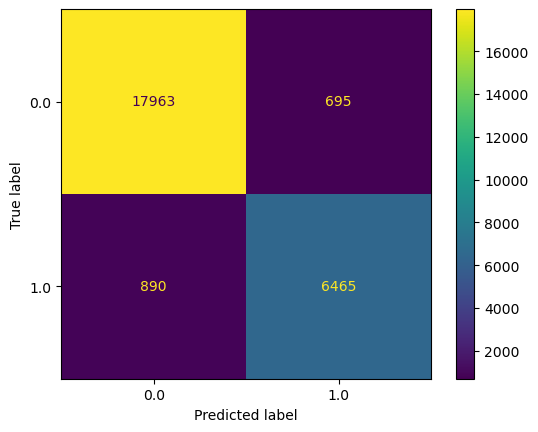
\includegraphics[width=0.3\textwidth]{vnn_confusion_matrix.png}
	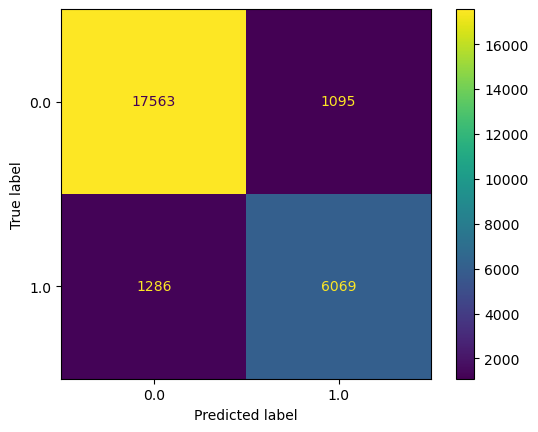
\includegraphics[width=0.3\textwidth]{svm_confusion_matrix.png}
	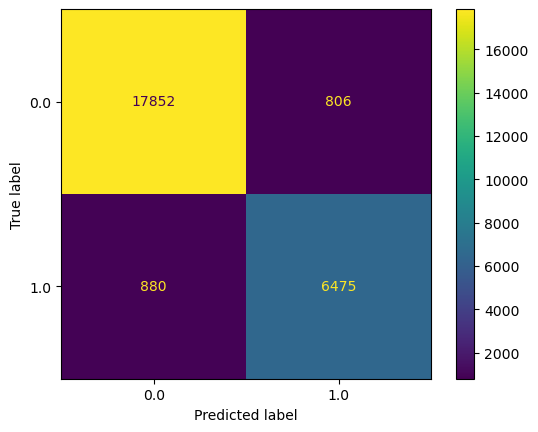
\includegraphics[width=0.3\textwidth]{rf_confusion_matrix.png}
\end{figure}
\end{document}